% !TEX root = ../../mat830_mckay.tex
\newpage
\section{Introduction}

The \mc Correspondence (pronounced mc-eye) is an umbrella for a family of correspondences linking finite groups, resolutions of singularities of algebraic varieties, Lie Algebras, Character Theory, Invariant Theory, Representations of Quivers, and Cohen-Macaulay modules. It will not be our goal to see any particular connection in depth, but rather a surface level introduction to these correspondences generally, with a strong emphasis on examples. \\

        \begin{nscenter}
        \begin{minipage}{0.8\textwidth}
        {\itshape ``The problem is to find a common origin of the ADE Classification Theorems, and to substitute a priori proofs to a posteriori verifications of the parallels of the classification.} \\
        \phantom{x}\hspace{1cm} -- V.I.~Arnold ,1976 \\
        \end{minipage}
        \end{nscenter}

The organizational scheme for the \mc Correspondence is the Coxeter-Dynkin diagrams. The Coxeter-Dynkin ADE diagrams classify objects in each of the areas above, plus subadditive functions, root systems, Weyl groups, String Theory, Cluster Algebras, etc.. An example theorem demonstrating the \mc Correspondence is the following, due to \mc, Auslander, Reiten, Artin, Verdier, Gonzalzez-Springber, Herzog, et al.,


\begin{thm}
Let $G$ be a small finite subgroup of $\SL_2(\C)$, acting linearly on $S= \C[x,y]$. Denote by $R=S^G$ the ring of invariants. Then there is a one-to-one correspondence between the following:
	\begin{itemize}
	\item Irreducible representations of G
	\item Indecomposable reflexive $R$-modules
	\item Irreducible Components of the exceptional fiber of minimal resolution of singularities of $\spec R$.
	\end{itemize}
These correspondences extend to isomorphisms between 
	\begin{itemize}
	\item the \mc Correspondence of $G$
	\item the Auslander-Reiten quiver of $R$
	\item the dual desingularization graph of $\spec R$. 
	\end{itemize}
\end{thm}



\newpage
% -------------------------
% Platonic Solids
% -------------------------
\section{Platonic Solids and Finite Groups of Matrices}


A Platonic solid is a regular, convex polyhedron, constructed by congruent regular polygonal faces with the same number of faces meeting at each vertex; that is, the platonic solids are defined by the property that the faces are each convex and pairwise congruent. The solids shown below are the only five solids satisfying these properties.
        \[
        \begin{tikzpicture}[thick,scale=2]
        \node at (0,-1,0) {Tetrahedron};
        \coordinate (V1) at (1.20821,-0.196544,0.0400412);
        \coordinate (V2) at (-0.557836,-0.981811,-0.474199);
        \coordinate (V3) at (-0.231484,0.978507,-0.699241);
        \coordinate (V4) at (-0.418887,0.199849,1.1334);
        
        \draw (V4) -- (V2);
        \draw (V1) -- (V3);
        \draw[dashed] (V1) -- (V4);
        \draw[fill=drk,opacity=0.6] (V1) -- (V2) -- (V3); %r
        \draw[fill=lght,opacity=0.6] (V2) -- (V3) -- (V4); %l
        \end{tikzpicture} \quad
	%
        \begin{tikzpicture}[thick,scale=1.25]
	\node at (-0.2,-1.6,0) {Cube};
        \coordinate (V1) at (1,1,1);
        \coordinate (V2) at (1,1,-1);
        \coordinate (V3) at (1,-1,1);
        \coordinate (V4) at (1,-1,-1);
        \coordinate (V5) at (-1,1,1);
        \coordinate (V6) at (-1,1,-1);
        \coordinate (V7) at (-1,-1,1);
        \coordinate (V8) at (-1,-1,-1);
        
        \draw[fill=drk,opacity=0.6] (V1) -- (V2) -- (V4) -- (V3) -- (V1);
        \draw[fill=lght,opacity=0.6] (V1) -- (V5) -- (V7) -- (V3) -- (V1);
        \draw[fill=med,opacity=0.6] (V1) -- (V5) -- (V6) -- (V2) -- (V1);
        \draw[dashed] (V4) -- (V8);
        \draw[dashed] (V6) -- (V8);
        \draw[dashed] (V7) -- (V8);
        \end{tikzpicture} \quad
	%
        \begin{tikzpicture}[thick,scale=2]
        \node at (0,-1.1,0) {Octahedron};
        \coordinate (V1) at (1,0,0);
        \coordinate (V2) at (-1,0,0);
        \coordinate (V3) at (0,1,0);
        \coordinate (V4) at (0,-1,0);
        \coordinate (V5) at (0,0,1);
        \coordinate (V6) at (0,0,-1);
        
        \draw[dashed] (V1) -- (V6);
        \draw[dashed] (V2) -- (V6);
        \draw[dashed] (V3) -- (V6);
        \draw[dashed] (V4) -- (V6);
        \draw[fill=drk,opacity=0.6]  (V2) -- (V3) -- (V5) -- (V2);
        \draw[fill=med,opacity=0.6]  (V2) -- (V4) -- (V5) -- (V2);
        \draw[fill=greet,opacity=0.6]  (V1) -- (V3) -- (V5) -- (V1);
        \draw[fill=lght,opacity=0.6]  (V1) -- (V4) -- (V5) -- (V1);
        \end{tikzpicture} 
        \]

        \[
        \begin{tikzpicture}[thick]
        \node at (0,-2.2,-0.1) {Dodecahedron};
        \coordinate (V1) at (0.826987,-0.308601,1.49025);
        \coordinate (V2) at (1.45166,0.942872,0.0607083);
        \coordinate (V3) at (0.399592,-1.6823,0.100911);
        \coordinate (V4) at (1.02426,-0.43083,-1.32864);
        \coordinate (V5) at (-1.02426,0.43083,1.32864);
        \coordinate (V6) at (-0.399592,1.6823,-0.100911);
        \coordinate (V7) at (-1.45166,-0.942872,-0.0607083);
        \coordinate (V8) at (-0.826987,0.308601,-1.49025);
        \coordinate (V9) at (-0.373296,-0.587966,1.58586);
        \coordinate (V10) at (0.637441,1.43696,-0.727196);
        \coordinate (V11) at (-0.637441,-1.43696,0.727196);
        \coordinate (V12) at (0.373296,0.587966,-1.58586);
        \coordinate (V13) at (0.917837,0.882852,1.17395);
        \coordinate (V14) at (0.226298,-1.33984,-1.07406);
        \coordinate (V15) at (-0.226298,1.33984,1.07406);
        \coordinate (V16) at (-0.917837,-0.882852,-1.17395);
        \coordinate (V17) at (1.30466,-0.984938,0.572506);
        \coordinate (V18) at (1.69073,-0.211486,-0.311002);
        \coordinate (V19) at (-1.69073,0.211486,0.311002);
        \coordinate (V20) at (-1.30466,0.984938,-0.572506);
        
        \draw[dashed] (V5) -- (V19) -- (V20) -- (V6) -- (V15) -- (V5);
        \draw[dashed] (V5) -- (V9) -- (V11) -- (V7) -- (V19) -- (V5);
        \draw[dashed] (V9) -- (V1) -- (V17) -- (V3) -- (V11) -- (V9);
        \draw[dashed] (V9) -- (V5) -- (V15) -- (V13) -- (V1) -- (V9);
        \draw[dashed] (V6) -- (V10) -- (V2) -- (V13) -- (V15) -- (V6);
        \draw[dashed] (V13) -- (V2) -- (V18) -- (V17) -- (V1) -- (V13);
        \draw[fill=med,opacity=0.6] (V7) -- (V16) -- (V8) -- (V20) -- (V19) -- (V7);
        \draw[fill=drk,opacity=0.6] (V11) -- (V3) -- (V14) -- (V16) -- (V7) -- (V11);
        \draw[fill=med,opacity=0.6] (V14) -- (V4) -- (V12) -- (V8) -- (V16) -- (V14);
        \draw[fill=lght,opacity=0.6] (V8) -- (V12) -- (V10) -- (V6) -- (V20) -- (V8);
        \draw[fill=med,opacity=0.6] (V18) -- (V2) -- (V10) -- (V12) -- (V4) -- (V18);
        \draw[fill=drk,opacity=0.6] (V17) -- (V18) -- (V4) -- (V14) -- (V3) -- (V17);
        \end{tikzpicture} \hspace{2cm}
        %
        \begin{tikzpicture}[thick]
        \node at (0,-2.4,-0.4) {Icosahedron};
        \coordinate (V1) at (1.59927,0.159038,1.01734);
        \coordinate (V2) at (-0.160427,-0.239969,1.88005);
        \coordinate (V3) at (0.173071,1.55995,1.07449);
        \coordinate (V4) at (0.7162,-1.60997,0.716232);
        \coordinate (V5) at (1.25575,1.30237,-0.587225);
        \coordinate (V6) at (-1.59143,0.656782,0.808647);
        \coordinate (V7) at (-1.25575,-1.30237,0.587225);
        \coordinate (V8) at (1.59143,-0.656782,-0.808647);
        \coordinate (V9) at (-0.7162,1.60997,-0.716232);
        \coordinate (V10) at (-0.173071,-1.55995,-1.07449);
        \coordinate (V11) at (0.160427,0.239969,-1.88005);
        \coordinate (V12) at (-1.59927,-0.159038,-1.01734);
        
        \draw[dashed] (V1) -- (V2) -- (V4) -- (V1);
        \draw[dashed] (V1) -- (V3) -- (V2) -- (V1);
        \draw[dashed] (V1) -- (V4) -- (V8) -- (V1);
        \draw[dashed] (V1) -- (V8) -- (V5) -- (V1);
        \draw[dashed] (V1) -- (V5) -- (V3) -- (V1);
        \draw[dashed] (V5) -- (V9) -- (V3) -- (V5);
        \draw[dashed] (V3) -- (V9) -- (V6) -- (V3);
        \draw[dashed] (V3) -- (V6) -- (V2) -- (V3);
        \draw[dashed] (V2) -- (V6) -- (V7) -- (V2);
        \draw[dashed] (V2) -- (V7) -- (V4) -- (V2);
	\draw[fill=lght,opacity=0.6] (V5) -- (V11) -- (V9) -- (V5);
        \draw[fill=lght,opacity=0.6] (V12) -- (V9) -- (V11) -- (V12);
        \draw[fill=lght,opacity=0.6] (V12) -- (V6) -- (V9) -- (V12);
	\draw[fill=med,opacity=0.6] (V8) -- (V11) -- (V5) -- (V8);
        \draw[fill=med,opacity=0.6] (V8) -- (V10) -- (V11) -- (V8);
        \draw[fill=med,opacity=0.6] (V12) -- (V11) -- (V10) -- (V12);
        \draw[fill=med,opacity=0.6] (V12) -- (V7) -- (V6) -- (V12);
        \draw[fill=med,opacity=0.6] (V12) -- (V10) -- (V7) -- (V12);
        \draw[fill=drk,opacity=0.6] (V4) -- (V7) -- (V10) -- (V4);
        \draw[fill=drk,opacity=0.6] (V4) -- (V10) -- (V8) -- (V4);
        \end{tikzpicture}
        \]


\begin{prop} \label{prop:allplatonic}
The solids above are the only possible Platonic solids.
\end{prop}

\pf Suppose a solid has faces with $p$ sides and $q$ faces meeting at each vertex. We write this as a pair $\{p,q\}$, called the Schl\"afli symbol. The external angles of each face add to $2\pi$ radians, as is the case with any convex polygon. Each exterior angle is then $\frac{2\pi}{p}$ radians. The internal angles are then $\pi - \frac{2\pi}{p}$. So around each vertex, the sum of the angles is $q(\pi - \frac{2\pi}{p})$. 
	\begin{table}[h]
	\centering
	\begin{tabular}{ccccc}
	$\{p,q\}$ & Name & $F$ & $E$ & $V$ \\ \hline
	$\{p,2\}$ & dihedron & 2 & $q$ & $q$ \\
	$\{2,q\}$ & hosohedron & $p$ & $p$ & 2 \\
	$\{3,3\}$ & tetrahedron & 4 & 6 & 4 \\
	$\{3,4\}$ & octahedron & 8 & 12 & 6 \\
	$\{4,3\}$ & cube & 6 & 12 & 8 \\
	$\{3,5\}$ & icosahedron & 20 & 30 & 12 \\
	$\{5,3\}$ & dodecahedron & 12 & 30 & 20
	\end{tabular}
	\end{table}
This angle cannot be larger than $2\pi$ as the faces are concave if and only if $\dfrac{2}{p} + \dfrac{2}{q}>1$, and we require convex faces. Furthermore, this sum cannot be $2\pi$ for then the solid would be flat, i.e. a tiling of the plane. Therefore, we have the relation
	\[
	q \left( \pi - \dfrac{2\pi}{p}\right)< 2\pi.
	\]
The integer solutions are $\{p,2\}$, $\{2,q\}$ or $\{3,3\}$, $\{3,4\}$, or $\{3,5\}$. Then Euler's Formula $V-E+F=1$ allows one to compute $V$, $E$, $F$, as found in the table. \qed \\


Notice that the above proof is merely a uniqueness proof and does \emph{not} show the existence of these solids. We shall prove existence by classifying the rotational symmetry groups of these solids. We shall find
	\begin{itemize}
	\item the dihedral group, $D_{2k}$, of the symmetries of the dihedron/hosohedron.
	\item the tetrahedral group, $\bbT$, of the 12 rotational symmetries of a tetrahedron. 
	\item the octahedral group, $\bbO$, of the 24 rotational symmetries of the octahedron.
	\item the icoahedral/dodecahedral group, $\bbI$, of 60 the rotational symmetries of the icosahedron/dodecahedron
	\end{itemize}
Note that dual pairs\footnote{The dual of a polyhedron $P$ has a vertex at the center of each face of $P$, and two vertices joined by an edge if the faces abut each other.} of polyhedra have the same rotational symmetry groups. Furthermore, these will all be familiar groups. For example, we shall find $\bbT \cong A_4$ and $\bbO \cong S_4$. This follows from the fact that symmetries of the faces of one polyhedron correspond to symmetries of the centers of their faces, and vice versa. For instance, the cube and the octahedron both have the same symmetry group, $\bbO \cong S_4$, because they are dual. From the table in Proposition~\ref{prop:allplatonic}, we can see that the dihedron and hosohedron are dual, the octahedron and cube are dual, the icosahedron and dodecahedron are dual, and the tetrahedron is self-dual. Finally, the groups $D_{2k}$, $\bbT$, $\bbO$, and $\bbI$, along with the cyclic groups $C_n$ for $n \in \N$, are the \emph{only} finite groups of rotations of $\R^3$.


\begin{thm}
Along with the degenerate case of the cyclic group $C_k$ for any $k \geq 1$ corresponding to rotation of $\R^3$ by $\dfrac{2\pi}{k}$, the groups $D_{2k}$, $\bbT$, $\bbO$, and $\bbI$ are all of the finite groups of rotations of $\R^3$. 
\end{thm}



% -------------------------
% Matrix Groups
% -------------------------
\subsection{Matrix Groups}

To classify the finite groups of rotational symmetries, we begin by recalling a few definitions.

\begin{dfn}[Orthogonal Group]
The orthogonal group, $O(n)$, is the set of all invertible orthogonal matrices, i.e. $O(n):= \{ A \in \GL_n(\R) \colon AA^T= I_n\}$.
\end{dfn}


\begin{ex}
The following are all orthogonal matrices:
	\[
	\begin{aligned}
	A&= \dfrac{1}{\sqrt{2}} \two{1}{1}{1}{-1} && && B&= \dfrac{1}{3} \three{2}{-2}{1}{1}{2}{2}{2}{1}{-2} \\
	P&= \begin{pmatrix} 0 & 1 & 0 & 0 \\ 0 & 0 & 0 & 1 \\ 1 & 0 & 0 & 0 \\ 0 & 0 & 1 & 0 \end{pmatrix} && && R&= \two{\cos\theta}{-\sin\theta}{\sin\theta}{\cos\theta}
	\end{aligned}
	\] \xqed
\end{ex}


A routine exercise verifies that the orthogonal group is also equivalent to any of the following:
	\[
	\begin{split}
	O(n)&:= \{ A \in \GL_n(\R) \colon AA^T= I_n\} \\
	&=\{ A \colon |Ax|=|x| \text{ for all }x \in \R^n\} \\
	&= \{A \colon Ax \cdot Ay = x \cdot y, \text{ for all }x,y \in \R^n\} \\
	&= \{ A \colon \text{ rows of }A\text{ form orthonormal basis for }\R^n\} \\
	&= \{ A \colon \text{ columns of }A\text{ form orthonormal basis for }\R^n\} \\
	&=\{ \text{set of linear isometries of }\R^n\}.
	\end{split}
	\]
Note that we have defined $O(n)$ in terms of the symmetric bilinear form $\langle A, B \rangle = AB^T$. Generally, if $\langle \cdot,\cdot \rangle$ is a symmetric bilinear form then you can define the orthogonal group of the form $\langle \cdot, \cdot \rangle$ to be $\{ A \in \GL(\R) \colon \langle Ax , Ay \rangle=\langle x, y \rangle \text{ for all }x,y \in \R\}$. Observe also that from the relation $AA^T=I_n$, we obtain $\det(AA^T)=1$. Recall that $\det(AB)=\det(A)\det(B)$, and $\det(A)=\det(A^T)$. It then follows that $\det(A)^2=1$, and then $\det A = \pm 1$.  A special subset of these matrices are our next group of interest. 


\begin{dfn}[Special Orthogonal Group]
The special orthogonal group, $\SO(n)$, is the subgroup of $O(n)$ of matrices having determinant 1, i.e. $\SO(n):= \{ A \in \GL_n(\R) \colon AA^T=I_n,\, \det A=1\}$. 
\end{dfn}


\begin{ex} \label{ex:so2}
The case of $n=1$ is dull, consisting only of the identity matrix. The case of $n=2$ is a bit more interesting. Suppose that $A= \two{a}{b}{c}{d} \in \SO(2) \subseteq O(2)$. Since $A \in O(2)$, we know that the columns of $A$ are orthogonal, giving
	\[
	\begin{pmatrix} a \\ c \end{pmatrix} \begin{pmatrix} b \\ d \end{pmatrix}^T=0.
	\]
A simple calculation shows that $\begin{pmatrix} a \\ c \end{pmatrix} \begin{pmatrix} c \\ -a \end{pmatrix}^T=0$. But then by linear independence, $\begin{pmatrix} b \\ d \end{pmatrix}$ must be a multiple of $\begin{pmatrix} c \\ -a \end{pmatrix}$. But these are also unit vectors, so the multiplier is $\pm 1$. This gives two possible cases for $A$: 
	\[
	A=\two{a}{-c}{c}{a} \text{ or } \two{a}{c}{c}{-a}.
	\]
Since $A \in \SO(2)$, we know that $\det A=1$. This gives $a^2+c^2=1$. Then we can find an angle $\theta \in [0,2\pi)$ so that $a= \cos \theta$ and $c= \sin \theta$. Using this in our possibilities above, we have
	\[
	A=\two{\cos\theta}{-\sin\theta}{\sin\theta}{\cos\theta} \text{ or } \two{\cos\theta}{\sin\theta}{\sin\theta}{-\cos\theta}
	\]
While the left matrix is an element of $\SO(2)$, the other has determinant $-1$. Therefore, we must have $A= \two{\cos\theta}{-\sin\theta}{\sin\theta}{\cos\theta}$, a rotation by $\theta$ counterclockwise about the origin. The second matrix on the right above corresponds to the reflection across the line at angle $\theta/2$ through the origin. Therefore, the group $\SO(2)$ is precisely the group of rotations in the plane. Similarly, $\SO(3)$ is the group of rotations for three-dimensional space, see Theorem~\ref{thm:eulerthm}. \xqed
\end{ex}


\begin{dfn}[Rotation of $\R^n$]
Let $n>2$. A rotation of $\R^n$ is a linear map $\phi: \R^n \to \R^n$ satisfying
	\begin{itemize}
	\item $\phi$ fixes a line $\ell$ through the origin
	\item $\phi \big|_{\ell^\perp}$ is a rotation of the subspace orthogonal to $\ell$
	\end{itemize}
\end{dfn}


Sometimes the definition of rotations of $\R^n$ is instead given as follows: a rotation of $\R^n$ is a linear operator if $T$ fixes a unit vector $p$, called a pole, and the  restriction of $T$ to $(\text{span}(p))^\perp \cong \R^2$ is a rotation of $\R^2$. We will make use of this alternate definition later. For now, we shall prove that the finite subgroups of linear isometries of the plane are a cyclic group or a dihedral group. 


\begin{thm}
The finite subgroups of linear isometries of the plane are a cyclic group or a dihedral group. 
\end{thm}

\pfsk If $G \subseteq \SO(2)$ is a finite group, then $G$ consists only of rotations by Example~\ref{ex:so2}. One can check that $G$ is generated by the rotation with smallest positive angle. Now if $G \subseteq O(2) \setminus \SO(2)$, then $G$ must contain a reflection $B$, and $G \cap \SO(2)= \langle A \rangle$ will be cyclic. One then verifies that $G= \{I,A, \ldots, A^{n-1}, B, BA, \ldots, BA^{n-1}\}$. \qed \\


\begin{cor}
$\SO(2)$ consists of the rotations of $\R^2$. 
\end{cor}

\pf By Example~\ref{ex:so2}, we know that $\SO(2)$ is contained in the group of rotations of $\R^2$. Since every rotation of $\R^2$ can be represented by a matrix in the form of $\two{\cos\theta}{-\sin\theta}{\sin\theta}{\cos\theta}$, the containment holds in the other direction. \qed \\


Note that $\SO(3)=\{\text{rotations of }\R^3\}$ but $\SO(n)$ strictly contains the rotations of $\R^n$ for $n \geq 4$. We now come to yet another theorem of Euler. 


\begin{thm}[Euler's Theorem] \label{thm:eulerthm}
	\[
	\SO(3)= \{\text{rotation of }\R^3\}
	\]
In particular, the composition of two rotations of $\R^3$ is another rotation.
\end{thm}

\pf Suppose $T$ is a rotation. We can find a basis for $\R^3$ of the form $\cB:=\{p,x_1,x_2\}$, where $p$ a pole for $T$ and $\{x_1, x_2\}$ is a basis for $\R^2= (\text{span}(p))^\perp$. With respect to the basis $\cB$, 
	\[
	[T]_\cB= 
	\begin{pmatrix}
	1 & 0 & 0 \\
	0 & \cos \theta & -\sin \theta \\
	0 & \sin \theta & \cos \theta
	\end{pmatrix} \in \SO(3).
	\]
Now let $A \in \SO(3)$. We need find a pole for $A$, i.e. a nonzero vector fixed by $A$. If this were the case, then $A$ must have 1 as an eigenvector. Using the fact that $\det A=1$, we have
	\[
	\begin{split}
	\det(A-I)&= \det(A)\det(A-I) \\
	&=\det(A^T)\det(A-I) \\
	&= \det(A^TA-A^T) \\
	&=\det(I-A^T) \\
	&=\det(I-A) \\
	&= \det(-(A-I)) \\
	&= (-1)^3 \det(A-I) \\
	&= - \det(A-I).
	\end{split}
	\]
Therefore, $\det(A-I)=0$. But then $A$ has a unit eigenvector, say $p$. The restriction of $A$ to $(\text{span}(p))^\perp$ still preserves the dot product, and so $A$ is a rotation of $\R^3$ by the $\SO(2)$ case. \qed \\


\begin{thm}
The finite subgroups of $\SO(3)$ are cyclic, dihedral, or the group of rotational symmetries of a tetrahedron, an octahedron, or an icosahedron (the symmetry groups of the Platonic solids).
\end{thm}

\pf Let $G \subseteq \SO(3)$ be finite with $|G|=N>1$, and define $P=\{\vec{p} \in \R^3 \colon \vec{p} \text{ pole of some }1\neq g \in G\}= \{ \vec{p} \in \R^3 \colon |\vec{p}|=1, g\vec{p}=g \text{ for some }g\neq 1\}$. We claim that $G$ acts on $P$, i.e. if $\vec{p} \in P$, $g \in G$, then $g\vec{p} \in P$. If $\vec{p}$ is a pole of $h \in G$, then $(ghg^{-1})(g\vec{p})=g\vec{p}$ since $h$ fixes $\vec{p}$. But then $g\vec{p}$ is a pole of $ghg^{-1}$. Observe each $1 \neq g \in G$ has two poles, so $|P|<\infty$. For $\vec{p} \in P$, let $G_{\vec{p}}:= \stab_{\vec{p}}=\{g \in G \colon \vec{p} \text{ pole of }g\} \cup \{1_G\}$. 

Now $G_{\vec{p}}$ is the set of all rotations with pole $\vec{p}$, and $G_{\vec{p}}$ is cyclic by the $n=2$ case. Furthermore, $G_{\vec{p}}$ is generated by the smallest nonzero rotation. Let $r_{\vec{p}}:= |G_{\vec{p}}|$, and $n_{\vec{p}}:=|O_{\vec{p}}|$, where $O_{\vec{p}}$ is the orbit of $\vec{p}$. So $r_{\vec{p}} n_{\vec{p}}=|G|$ by the Orbit-Stabilizer Theorem. We count pairs $(\vec{p},g)$, where $\vec{p}$ is a pole of $g \neq 1$. Now each $g$ has two poles so
	\[
	|\{ (\vec{p},g) \colon \vec{p} \in P, g\vec{p}=\vec{p}, g \neq 1\}| = 2 (N-1) = \sum_{\vec{p} \in P} r_{\vec{p}} - 1
	\]
where the last equality follows since $G_{\vec{p}}$ is the set of $g$'s with pole $\vec{p}$. Replacing $r_{\vec{p}}$ with $N/n_{\vec{p}}$, we obtain 
	\[
	2N-2 = \sum_{\vec{p} \in P} \dfrac{N}{n_{\vec{p}}} -1 = \sum_{\text{orbits }O_{\vec{p}}} n_{\vec{p}} \left(\dfrac{N}{n_{\vec{p}}} -1 \right) = \sum_{\text{orbits }O_{\vec{p}}} N - \dfrac{N}{r_{\vec{p}}}.
	\]
But then we have
	\[
	2 - \dfrac{2}{N} = \sum_{i=1}^k \left( 1 - \dfrac{1}{r_i}\right),
	\]
where we have labeled the orbits $O_1,\ldots,O_k$ and $r_i= |G_{\vec{p}_i}|$. This equation is known as L\"uroth's Equation. 

L\"uroth's equation implies that $k \leq 3$, as each term on the right hand side is at least $1/2$ and the left hand side is less than 2. If $k=1$, then there is a unique orbit or poles and thus $2- \frac{2}{N}= 1- \frac{1}{r}$. But the left hand side is at least 1, while the right hand side is less than 1, a contradiction. Now if $k=2$, then there are two orbits of poles so that
	\[
	\left(1-\dfrac{1}{r_1}\right) + \left(1-\dfrac{1}{r_2}\right)= 2-\dfrac{2}{N} \Longleftrightarrow \dfrac{1}{r_1} + \dfrac{1}{r_2} = \dfrac{2}{N} \Longleftrightarrow n_1+n_2 =2,
	\]
where the last equivalence follows since $r_in_i=N$, where $n_i=|O_i|$. But then each orbit is a singleton set, implying there are two poles. Furthermore, $r_i=N$ for $i=1,2$ so that every group element fixes both poles. Then $G \cong C_N$ by the $n=2$ case. In the case of $k=3$, we have
	\[
	\dfrac{1}{r_1} + \dfrac{1}{r_2} + \dfrac{1}{r_3} = 1 + \dfrac{2}{N}>1.
	\]
The number of algebraic possibilities are limited. We can assume $r_1 \leq r_2 \leq r_3$ and so $r_1<3$. The solutions are $(2,2,k)$ for any $k \geq 2$, $(2,3,3)$, $(2,3,4)$, $(2,3,5)$. We can construct the polyhedron in each case. 
	\begin{itemize}
	\item  $(2,2,k)$: \enskip We have $\frac{1}{2}+\frac{1}{2}+\frac{1}{k}=1+\frac{2}{N}$, so $N=2k$. But then there are two orbits of size $k$ and one of size 2, say $O_3=\{\vec{p},\vec{p}' \}$. Half the elements of $G$, i.e. $k$ elements, fix $\vec{p}$ and $\vec{p}'$, while the remaining elements swap the elements. But then $G \cong D_k$.  
	\item $(2,3,5)$: \enskip We have $\frac{1}{2}+\frac{1}{3}+\frac{1}{5}=1+\frac{2}{N}$ so that $N=60$. The orbits have sizes 30, 20, and 12. Let $V=O_3$ be the orbit of size 12. Choose $p \in V$ to be the north pole, and let $H=G_{\vec{p}}$ be the stabilizer of $p$. We have $|H|= \frac{60}{12}=5$. In particular, $H$ is cyclic with order 5. Now $H$ (with order 5) acts on $V$ (of order 12), fixing $\vec{p}$ and $-\vec{p}$. But then the orbits have size 1, 1, 5, and 5. Now $V$ is the set of vertices of the icosahedron. 
		\[
		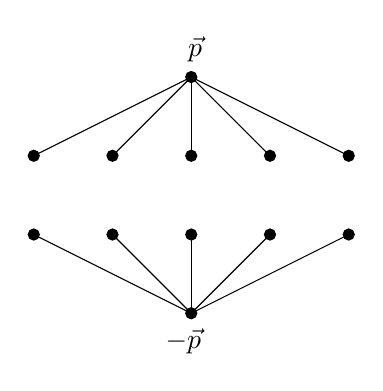
\begin{tikzpicture}
		\node at (3.05,1.35) {$\vec{p}$};
		\node at (2.9,-2.35) {$-\vec{p}$};
		\filldraw[black] (3,1) circle (2pt);
		\filldraw[black] (3,-2) circle (2pt);
		
		\filldraw[black] (1,0) circle (2pt);
		\filldraw[black] (2,0) circle (2pt);
		\filldraw[black] (3,0) circle (2pt);
		\filldraw[black] (4,0) circle (2pt);
		\filldraw[black] (5,0) circle (2pt);

		\filldraw[black] (1,-1) circle (2pt);
		\filldraw[black] (2,-1) circle (2pt);
		\filldraw[black] (3,-1) circle (2pt);
		\filldraw[black] (4,-1) circle (2pt);
		\filldraw[black] (5,-1) circle (2pt);
		
		\draw (1,0) -- (3,1);
		\draw (2,0) -- (3,1);
		\draw (3,0) -- (3,1);
		\draw (4,0) -- (3,1);
		\draw (5,0) -- (3,1);
		
		\draw (1,-1) -- (3,-2);
		\draw (2,-1) -- (3,-2);
		\draw (3,-1) -- (3,-2);
		\draw (4,-1) -- (3,-2);
		\draw (5,-1) -- (3,-2);
		\end{tikzpicture}
		\]
	\item The cases of $(2,3,3)$ and $(2,3,4)$ are handled the same as the case above. 
	\end{itemize}
\qed \\


\begin{cor}
The finite subgroups of $\SO(3)$ have presentations 
	\[
	\begin{split}
	\mathbb{C}_n&= \langle x \;|\; x^n=1 \rangle \\
	\mathbb{D}_n&= \langle x,y \;|\; x^2=y^n=(xy)^2=1 \rangle \\
	\mathbb{T}&= \langle x,y \;|\; x^2=y^3=(xy)^3=1 \rangle \\
	\bbO&= \langle x,y \;|\; x^2=y^3=(xy)^4=1 \rangle \\
	\mathbb{I}&= \langle x,y \;|\; x^2=y^3=(xy)^5=1 \rangle
	\end{split}
	\]
\end{cor}

\pfsk Suppose we have the Sch\"afli symbol $\{p,q\}$, i.e. each face has $p$ sides, and $q$ meet at each vertex. Fix a vertex, and let $\tau$ be rotation by $2\pi/q$ around this vertex. But then $|\tau|=q$. Also, fix an edge incident to our vertex, and let $\sigma$ be the rotation swapping the ends of this edge. Then $|\sigma|=2$. 

% Give image vertex with 5 whell spoked and arrow between 2 spokes with 2 or i? Give upper right edge color, the specified one, along it label \sigma . This has bunny with head along chosen edge. Give image to right of sigma, then give arrow connecting to similar diagram labeled tau and rotate the same image and again by sigma till back to original with bunny facing origin feet on original edge. 

Focus on the face fo the right of our edge, and consider $\sigma\tau$. This rotates the face by $2\pi//p$. So we must have $|\sigma\tau|=p$, and we have elements $\sigma$, $\tau$ satisfying $\sigma^2=\tau^q=(\sigma\tau)^p=1$. One needs to check that $\sigma$, $\tau$ generate $G$, and that
	\[
	|\langle x,y \;|\; x^2=y^q=(xy)^p=1 \rangle| = |G|.
	\]
\qed \\

 
\begin{cor}
We have isomorphisms $\mathbb{T} \cong A_4$, $\bbO \cong S_4$, $\mathbb{I} \cong A_5$. 
\end{cor}

 Note that the group $\langle x,y \;|\; x^r=y^s=(xy)^t=1\rangle$ is \emph{only} finite in the cases above. Associate to this the graph $T_{r,s,t}$, shown below.
 	\[
	\begin{tikzpicture}
	\foreach \Point in {(-2,1.5), (-1,1), (-2,3), (-1,2.5), (1,3)}{
    \node at \Point {\textbullet};
}
	\end{tikzpicture}
	\]
	% r on bottom left, t on bottom right and s above, cnetral node counted each time

with total $+s+t-2$ vertices. 

$C_n$: $(n,1,n)$ give horizontal line with dots, the dynkin $A_{2n-1}$
$D_n$: $(2,n,2)$  $D_{n+1}$
$T$: $(2,3,3)$ $E_6$
$O(2,3,4)$ $E_7$
$I(2,3,5)$ $E_8$

These are the ADE Coxeter-Dynkin diagrams. 














Our next goal is to classify the finite subgroups of $\SL_2(\C)$. We travel from $\SO(3)$, to $\SU(2)$, onto $\SL_2(\C)$. 

\begin{dfn}[Unitary Group]
$U(n):= \{A \in \GL_n(\C) \colon A^*A=I_n\}$, where $A^*=\ov{A^T}$. But this is also $\{A \colon |Ax|=|x|\}$ Euclidean norm $=\{ A \colon (Ax)^*(Ay)=x^*y\}$ i.e. $A$ preserves the Hermitian inner product $\langle x,y \rangle = x^*y$. That is the $\{A \colon \text{rows/col of }A \text{ are orthogonal basis for }\C^n\}$. 
\end{dfn}

As before $U(n)$ can be described as the set of matrices preserving an arbitrary Hermitian inner product. 

\begin{dfn}[Special Unitary Group]
$\SU(n):=\{A \in U(n) \colon \det A=1\}$. 
\end{dfn}








\begin{lem}
Every finite subgroup of $\GL_n(\C)$ is conjugate to a finite subgroup of $U(n)$. In particular, every subgroup of $\SL_n(\C)$ is conjugate to a finite subgroup of $\SL_n(\C)$ and $\SU(n)$. 
\end{lem}

\pf Let $G \subseteq \GL_n(\C)$ be a finite subgroup. We construct a new Hermitian inner product on $\C^n$ so that a given finite group $G$ preserves the product. Define $\langle u,v \rangle:= \frac{1}{|G|} \sum_{g \in G} (gu)^*(gv)$. Then for any $h \in G$, $u,v \in \C^n$,
	\[
	\langle hu,hv \rangle= \frac{1}{|G|} \sum_{g \in G} (ghu)^*(ghv)= \frac{1}{|G|} \sum_{k \in G} (ku)^*(kv)=\langle u,v \rangle. 
	\]




Let $\cB=\{b_1,\ldots,b_n\}$ be an orthonormal basis with respect to the form $\langle \;,\;\rangle$ for $\C^n$, and let $\rho: \C^n \to \C^n$ be the change of basis taking the standard basis to $B$. Then 
	\[
	\langle \rho e_i,\rho e_j \rangle= \langle b_i,b_j\rangle = \begin{cases} 1, & i=j \\ 0, & i\neq j \end{cases}.
	\]
It follows from linearity that $\langle \rho e_i,\rho e_j \rangle= u^*v$. Then for any $g \in G$, we claim that $\rho^{-1}g \rho \in U(n)$. It is sufficient to show that $\rho^{-1}g\rho$ preserves the usual Hermitian inner product. We have
	\[
	u^*v= \langle \rho u, \rho v \rangle= \langle g\rho u, g\rho v \rangle = (\rho^{-1}g\rho u)^* (\rho^{-1}h\rho v),
	\]
since $\rho^{-1}$ is the opposite change of basis. Therefore, $\rho^{-1} G \rho \subseteq U(n)$. As conjugation preserves the dot product, if $G \subseteq \SL_n(\C)$, then $\rho^{-1}G\rho \subseteq \SU(n)$. \qed \\


In order to classify the finite subgroups of $\SL_2(\C)$, we need to understand $\SU(2)$. We know
	\[
	\begin{split}
	\SU(2)= \left\{ A = \two{\alpha}{\beta}{\gamma}{\delta} \;\bigg|\; A^*=A^{-1}, \det A=1 \right\}= \left\{ \two{\alpha}{-\beta}{\ov{\beta}}{\ov{\alpha}} \;\bigg|\; \alpha,\beta \in \C, |\alpha|^2+|\beta|^2=1 \right\}.
	\end{split}
	\]
To relate $\SO(3)$ and $\SU(2)$, we define a map $\pi: \SU(2) \to \SO(3)$. The group $\SO(3)$ is the group of symmetries of the unit sphere $S^2$. We define an action of $\SU(2)$ on $S^2$ by rotations. Since $\SU(2)$ acts naturally on $\C^2$, i.e. $2\times 2$ matrices, hence on $\bP^1_\C=\C^2/\sim$ (since the determinant is 1). 

% Stereographic projection picture
	\[
	\begin{tikzpicture}
	
	\end{tikzpicture}
	\]

Topologically, $\P^1_\C$ is a real 2-sphere. But this gives a natural map $\pi: \SU(2) \to \SO(3)$, which one routinely verifies is a group homomorphism, and $-I_2$ acts trivially. In fact, one can verify that $\ker \pi= \{\pm I_2\}$. Therefore, $\pi$ is a two-to-one cover of $\SO(3)$. 


\begin{lem}
The only element of order 2 in $\SU(2)$ is $-I_2$.
\end{lem}

\pfsk Use the explicit form of the elements of $\SU(2)$. \qed \\


\begin{thm}
A finite subgroup of $\SU(2)$ is either cyclic of odd order or a double cover of a finite subgroup of $\SO(3)$. 
\end{thm}

\pf Let $\Gamma \subseteq \SU(2)$ be a finite subgroup. If $\Gamma$ has odd order, then by Lagrange's Theorem $\Gamma$ has no elements of order 2. Then $\Gamma \cap \ker \pi= \{I_2\}$ so that $\pi\big|_\Gamma: \Gamma \to \SO(3)$ maps $\Gamma$ bijectively to a finite subgroup of $\SO(3)$. The only such of odd order are the cyclic groups. If $\Gamma$ has even order, then by Cauchy's Theorem $\Gamma$ contains an element of order 2. Then $\ker \pi \subseteq \Gamma$ so that $\pi\big|_\Gamma$ is a two-to-one homomorphism onto a finite subgroup of $\SO(3)$. \qed \\


\begin{thm}
The finite subgroups of $\SL_2(\C)$, up to conjugacy, are
	\[
	\begin{split}
	\C_n=\left\langle \two{\omega}{0}{0}{\omega^{-1}} \right\rangle,
	B\cD_n:= \left\langle \C_{2n}, \two{0}{i}{i}{0} \right\rangle \\
	B\cT:= \left\langle B\cD_2, \dfrac{1}{\sqrt{2}} \two{\omega_8}{\omega_8^3}{\omega_8}{\omega_8^7} \right\rangle \\
	B\cO&= \left\langle B\cT, \two{\omega_8^3}{0}{0}{\omega_8^5} \right\rangle \\
	B\bbI= \left\langle ????\right\rangle
	\end{split}
	\]
where $\omega$ is a primitive $n$\tss{th} root of unity. The group $B\cD_n$ is the binary dihedral group of order $4n$, $B\cT$ is the binary tetrahedral group of order 24, $B\cO$ the binary octahedral group of order 48, and $B\bbI$ the binary icosahedral group of order 120. 
\end{thm}


The explicit generators come from the quaternionic description of $\pi$. There is also a classification of finite subgroups of $\GL_2(\C)$, coming from the extension of groups
	\[
	1 \ma{} \SL_2(\C) \ma{} \GL_2(\C) \ma{\det} \C^\times \ma{} 1.
	\]
So any $G \subseteq \GL_2(\C)$ is an extension of $G \cap \SL_2(\C)$ by a finite subgroup of $\C^\times$---which are cyclic. Though it takes a certain amount of work, one can classify the finite subgroups of $\SL_3(\C)$ using $A \in \SL_3(\C)$
	\[
	A \in \SL_3(\C) \rightsquigarrow \left( \begin{tabular}{c|ccc} $\det B^{-1}$ & & \\ \hline & & \\ & $B$ & \\ & & \end{tabular} \right), B \in \GL_2(\C).
	\]


























